\documentclass[]{article}
\usepackage{lmodern}
\usepackage{amssymb,amsmath}
\usepackage{ifxetex,ifluatex}
\usepackage{fixltx2e} % provides \textsubscript
\ifnum 0\ifxetex 1\fi\ifluatex 1\fi=0 % if pdftex
  \usepackage[T1]{fontenc}
  \usepackage[utf8]{inputenc}
\else % if luatex or xelatex
  \ifxetex
    \usepackage{mathspec}
  \else
    \usepackage{fontspec}
  \fi
  \defaultfontfeatures{Ligatures=TeX,Scale=MatchLowercase}
\fi
% use upquote if available, for straight quotes in verbatim environments
\IfFileExists{upquote.sty}{\usepackage{upquote}}{}
% use microtype if available
\IfFileExists{microtype.sty}{%
\usepackage{microtype}
\UseMicrotypeSet[protrusion]{basicmath} % disable protrusion for tt fonts
}{}
\usepackage[margin=1in]{geometry}
\usepackage{hyperref}
\hypersetup{unicode=true,
            pdftitle={Study example},
            pdfauthor={Alexandros Rekkas and Peter R. Rijnbeek},
            pdfborder={0 0 0},
            breaklinks=true}
\urlstyle{same}  % don't use monospace font for urls
\usepackage{color}
\usepackage{fancyvrb}
\newcommand{\VerbBar}{|}
\newcommand{\VERB}{\Verb[commandchars=\\\{\}]}
\DefineVerbatimEnvironment{Highlighting}{Verbatim}{commandchars=\\\{\}}
% Add ',fontsize=\small' for more characters per line
\usepackage{framed}
\definecolor{shadecolor}{RGB}{248,248,248}
\newenvironment{Shaded}{\begin{snugshade}}{\end{snugshade}}
\newcommand{\AlertTok}[1]{\textcolor[rgb]{0.94,0.16,0.16}{#1}}
\newcommand{\AnnotationTok}[1]{\textcolor[rgb]{0.56,0.35,0.01}{\textbf{\textit{#1}}}}
\newcommand{\AttributeTok}[1]{\textcolor[rgb]{0.77,0.63,0.00}{#1}}
\newcommand{\BaseNTok}[1]{\textcolor[rgb]{0.00,0.00,0.81}{#1}}
\newcommand{\BuiltInTok}[1]{#1}
\newcommand{\CharTok}[1]{\textcolor[rgb]{0.31,0.60,0.02}{#1}}
\newcommand{\CommentTok}[1]{\textcolor[rgb]{0.56,0.35,0.01}{\textit{#1}}}
\newcommand{\CommentVarTok}[1]{\textcolor[rgb]{0.56,0.35,0.01}{\textbf{\textit{#1}}}}
\newcommand{\ConstantTok}[1]{\textcolor[rgb]{0.00,0.00,0.00}{#1}}
\newcommand{\ControlFlowTok}[1]{\textcolor[rgb]{0.13,0.29,0.53}{\textbf{#1}}}
\newcommand{\DataTypeTok}[1]{\textcolor[rgb]{0.13,0.29,0.53}{#1}}
\newcommand{\DecValTok}[1]{\textcolor[rgb]{0.00,0.00,0.81}{#1}}
\newcommand{\DocumentationTok}[1]{\textcolor[rgb]{0.56,0.35,0.01}{\textbf{\textit{#1}}}}
\newcommand{\ErrorTok}[1]{\textcolor[rgb]{0.64,0.00,0.00}{\textbf{#1}}}
\newcommand{\ExtensionTok}[1]{#1}
\newcommand{\FloatTok}[1]{\textcolor[rgb]{0.00,0.00,0.81}{#1}}
\newcommand{\FunctionTok}[1]{\textcolor[rgb]{0.00,0.00,0.00}{#1}}
\newcommand{\ImportTok}[1]{#1}
\newcommand{\InformationTok}[1]{\textcolor[rgb]{0.56,0.35,0.01}{\textbf{\textit{#1}}}}
\newcommand{\KeywordTok}[1]{\textcolor[rgb]{0.13,0.29,0.53}{\textbf{#1}}}
\newcommand{\NormalTok}[1]{#1}
\newcommand{\OperatorTok}[1]{\textcolor[rgb]{0.81,0.36,0.00}{\textbf{#1}}}
\newcommand{\OtherTok}[1]{\textcolor[rgb]{0.56,0.35,0.01}{#1}}
\newcommand{\PreprocessorTok}[1]{\textcolor[rgb]{0.56,0.35,0.01}{\textit{#1}}}
\newcommand{\RegionMarkerTok}[1]{#1}
\newcommand{\SpecialCharTok}[1]{\textcolor[rgb]{0.00,0.00,0.00}{#1}}
\newcommand{\SpecialStringTok}[1]{\textcolor[rgb]{0.31,0.60,0.02}{#1}}
\newcommand{\StringTok}[1]{\textcolor[rgb]{0.31,0.60,0.02}{#1}}
\newcommand{\VariableTok}[1]{\textcolor[rgb]{0.00,0.00,0.00}{#1}}
\newcommand{\VerbatimStringTok}[1]{\textcolor[rgb]{0.31,0.60,0.02}{#1}}
\newcommand{\WarningTok}[1]{\textcolor[rgb]{0.56,0.35,0.01}{\textbf{\textit{#1}}}}
\usepackage{graphicx,grffile}
\makeatletter
\def\maxwidth{\ifdim\Gin@nat@width>\linewidth\linewidth\else\Gin@nat@width\fi}
\def\maxheight{\ifdim\Gin@nat@height>\textheight\textheight\else\Gin@nat@height\fi}
\makeatother
% Scale images if necessary, so that they will not overflow the page
% margins by default, and it is still possible to overwrite the defaults
% using explicit options in \includegraphics[width, height, ...]{}
\setkeys{Gin}{width=\maxwidth,height=\maxheight,keepaspectratio}
\IfFileExists{parskip.sty}{%
\usepackage{parskip}
}{% else
\setlength{\parindent}{0pt}
\setlength{\parskip}{6pt plus 2pt minus 1pt}
}
\setlength{\emergencystretch}{3em}  % prevent overfull lines
\providecommand{\tightlist}{%
  \setlength{\itemsep}{0pt}\setlength{\parskip}{0pt}}
\setcounter{secnumdepth}{5}
% Redefines (sub)paragraphs to behave more like sections
\ifx\paragraph\undefined\else
\let\oldparagraph\paragraph
\renewcommand{\paragraph}[1]{\oldparagraph{#1}\mbox{}}
\fi
\ifx\subparagraph\undefined\else
\let\oldsubparagraph\subparagraph
\renewcommand{\subparagraph}[1]{\oldsubparagraph{#1}\mbox{}}
\fi

%%% Use protect on footnotes to avoid problems with footnotes in titles
\let\rmarkdownfootnote\footnote%
\def\footnote{\protect\rmarkdownfootnote}

%%% Change title format to be more compact
\usepackage{titling}

% Create subtitle command for use in maketitle
\providecommand{\subtitle}[1]{
  \posttitle{
    \begin{center}\large#1\end{center}
    }
}

\setlength{\droptitle}{-2em}

  \title{Study example}
    \pretitle{\vspace{\droptitle}\centering\huge}
  \posttitle{\par}
    \author{Alexandros Rekkas and Peter R. Rijnbeek}
    \preauthor{\centering\large\emph}
  \postauthor{\par}
      \predate{\centering\large\emph}
  \postdate{\par}
    \date{2020-05-25}


\begin{document}
\maketitle

{
\setcounter{tocdepth}{2}
\tableofcontents
}
\hypertarget{introduction}{%
\section{Introduction}\label{introduction}}

Generalizability of an overall result found in a study and applicability
to a specific patient move in opposite directions. When patients differ
from one another in many key determinants of the outcome of
interest--and consequently in the potential benefits and harms of
therapy--it can be unclear to whom the overall average benefit-harm
trade-offs actually apply. Precision medicine aims to tailor treatment
to individual patients. As such, analysis of heterogeneity of treatment
effect (HTE), i.e.~non-random variation in the direction or magnitude of
a treatment effect for individuals within a population, is the
cornerstone of precision medicine; its goal is to predict the optimal
treatments at the individual level, accounting for an individual's risk
for harm and benefit outcomes.

This vignette describes the application of a risk modeling predictive
approach to the assessment of treatment effect heterogeneity (HTE) using
the \texttt{RiskStratifiedEstimation} package. The method involves 4
main steps summarized in Figure \ref{workflow}:

\begin{itemize}
\tightlist
\item
  \textbf{Definition of the problem:} For this step we need to define
  (at least) 3 essential cohorts: (1) the treatment cohort, containing
  the set of patients receiving the treatment treatment interest; (2)
  the comparator cohort, containing the set of patients receiving the
  comparator cohort; (3) the outcome cohort(s), containing the set of
  patients having the outcome(s) of interest.
\item
  \textbf{Identification of the database:} We need to define the
  database(s) on which we will assess treatment effect heterogeneity. We
  need to make sure that the cohorts created contain enough patients to
  proceed with the application of the method.
\item
  \textbf{Prediction step:} Combine the treatment and comparator cohorts
  into a single cohort for prediction and then provide the settings
  required for prediction based on the \texttt{PatientLevelPrediction}
  package. This means that we need to define the time-at-risk (time
  interval within which we want to predict), the set of predictive
  covariates and the prediction algorithm to be used (along with its
  settings).
\item
  \textbf{Estimation step:} Divide the treatment population in a
  pre-specified number of equal-sized strata based on baseline risk and
  estimate the absolute and relative treatment effects.
\end{itemize}

\begin{figure}
\centering
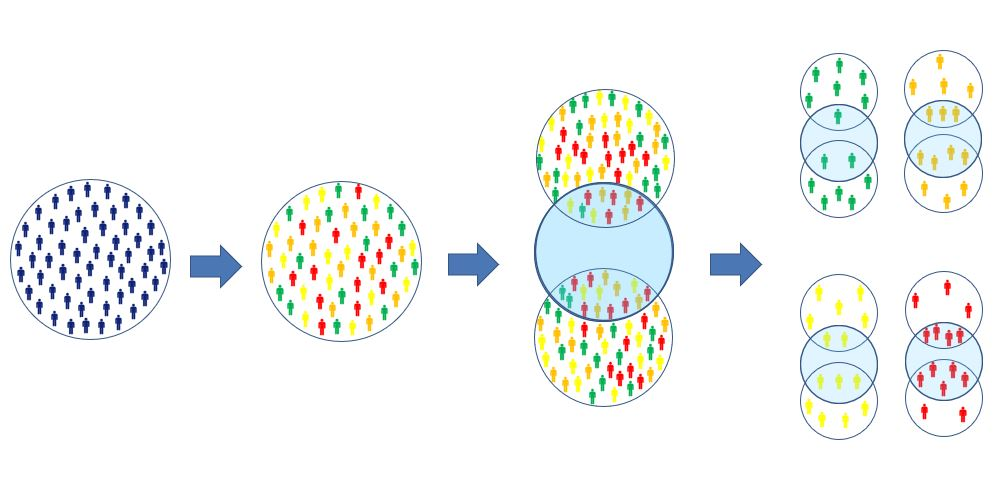
\includegraphics{rsee_workflow.JPG}
\caption{RiskStratifiedEstimation package workflow \label{workflow}}
\end{figure}

\hypertarget{study-specification-and-database-selection}{%
\section{Study specification and database
selection}\label{study-specification-and-database-selection}}

For the current demonstration we consider some of the treatments and
outcomes assessed in the Large-scale Evidence Generation in Network of
Databases (LEGEND) study for hypertension. The treatment cohort contains
patients with a hypertension diagnosis within the database that receive
angiotensin-converting enzyme (ACE) inhibitors, followed from the time
of initiation until the time of cessation. The comaparator cohort
contains the set of patients within the database with a hypertension
diagnosis that receive beta blockers. We also consider 2 outcome
cohorts. The first contains all patients found in the database that have
at least one occurrence of cardiovascular disease (CVD). The second
contains all patients with an occurrence of cough. We consider CVD as
the main outcome of interest that we are trying to prevent in the study
and cough as a common side-effect of ACE-inhibitors. Cohort definitions
are available online \href{https://github.com/OHDSI/Legend}{here}.

After the defining the problem we need to define the database on which
we will assess treatment effect heterogeneity. We need to make sure that
the defined cohorts are of adequate size to perform the analysis. This
is relevant to all cohorts defined. Very small treatment or comparator
cohorts reduce the power of our analyses restricting the minimum
detectable differences. Due to the stratified approach of the framework
this aspect is very relevant. The size of the outcome cohorts is also
very important for both the prediction and the estimation steps. In the
former case, low events per variable may limit the prediction
performance, while in the latter case, risk stratification may result to
in very few or even no observed cases in the lower strata.

\hypertarget{study-implementation}{%
\section{Study implementation}\label{study-implementation}}

\hypertarget{cohort-instantiation}{%
\subsection{Cohort instantiation}\label{cohort-instantiation}}

Similar to PLP package

\hypertarget{study-script-creation}{%
\subsection{Study script creation}\label{study-script-creation}}

In this section we assume that our cohorts have been created and have
been extracted using a specific database. Then we can proceed with the
creation of the script that will perform the defined study. For this
part 7 types of input need to be created:

\begin{itemize}
\tightlist
\item
  connection details
\item
  anlaysis settings
\item
  database settings
\item
  Settnigs for getting the data
\item
  covariate settings
\item
  population settings
\item
  run settings
\end{itemize}

\hypertarget{analysis-settnigs}{%
\subsubsection{Analysis settnigs}\label{analysis-settnigs}}

The analysis settings refer to information that define the structure of
the study and can be used to identify it. The analysis id is
a--pereferably--unique identifier of the present study. The treatment
cohort id refers to the unique identifier of the treatment cohort
definition. In our case, that is \(1001\) and refers to the extracted
hypertensive patients receving ACE-inhibitors. The comparator cohort id
refers to the unique identifier of the comparator cohort. In our case
this is \(1002\) and refers to the extracted cohort of hypertensive
patients receiving beta blockers; the outcome ids that refer to the
unique identifiers of the outcome cohorts. A very important
characteristic of the analysis settings is the analysis matrix, that
dictates which comparisons are to be made. The columns of this square
boolean matrix refer to risk stratification outcomes and the rows to
estimation outcomes. Therefore, the default diagonal matrix defines the
following analyses:

\begin{itemize}
\tightlist
\item
  Within strata of CVD risk estimate relative and absolute treatment
  effects of CVD events.
\item
  Within strata of acute myocardial infarction risk estimate relative
  and absolute treatment effects of acute myocardial infarction events.
\end{itemize}

We can create the analysis settings using the following code:

\begin{Shaded}
\begin{Highlighting}[]
\NormalTok{analysisSettings <{-}}\StringTok{ }\KeywordTok{createAnalysisSettings}\NormalTok{ (}
  \DataTypeTok{analysisId =} \StringTok{"vignette\_demonstration"}\NormalTok{,}
  \DataTypeTok{analysisType =} \StringTok{"stratifyByPs"}\NormalTok{,}
  \DataTypeTok{description =} \StringTok{"description text"}\NormalTok{,}
  \DataTypeTok{treatmentCohortId =} \DecValTok{1001}\NormalTok{,}
  \DataTypeTok{comparatorCohortId =} \DecValTok{1002}\NormalTok{,}
  \DataTypeTok{outcomeIds =} \KeywordTok{c}\NormalTok{(}\DecValTok{131}\NormalTok{, }\DecValTok{102}\NormalTok{),}
  \DataTypeTok{analysisMatrix =} \KeywordTok{diag}\NormalTok{(}\DecValTok{2}\NormalTok{)),}
\NormalTok{verbosity =}\StringTok{ "INFO"}\NormalTok{,}
\NormalTok{saveDirectory =}\StringTok{ "path/to/save/directory"}
\ErrorTok{)}
\end{Highlighting}
\end{Shaded}

\hypertarget{connection-details}{%
\subsubsection{Connection details}\label{connection-details}}

We need to define our connection details that will be used to connect to
the database we have access to in order to construct extract the data
objects required for our analyses. They can be created from:

\begin{Shaded}
\begin{Highlighting}[]
\NormalTok{connectionDetails <{-}}\StringTok{ }\NormalTok{DatabaseConnector}\OperatorTok{::}\KeywordTok{createConnectionDetails}\NormalTok{(}
  \DataTypeTok{dbms =}\NormalTok{ dbms,}
  \DataTypeTok{server =}\NormalTok{ server,}
  \DataTypeTok{user =} \StringTok{"joe"}\NormalTok{,}
  \DataTypeTok{password =} \StringTok{"secret"}\NormalTok{,}
  \DataTypeTok{port =}\NormalTok{ port}
\NormalTok{)}
\end{Highlighting}
\end{Shaded}

\hypertarget{database-settings}{%
\subsubsection{Database settings}\label{database-settings}}

The database settings contain relevant information on the database we
want to access. These refer to the database schema based on which we
extract our data along with the tables where the cohorts of interest are
stored. Note that we also need to create a table containing the merged
treatment and comparator cohorts that will be used to derive the
prediction models (requires write permission). Database settings can be
created from:

\begin{Shaded}
\begin{Highlighting}[]
\NormalTok{databaseSettings <{-}}\StringTok{ }\KeywordTok{createDatabaseSettings}\NormalTok{(}
  \DataTypeTok{cdmDatabaseSchema =} \StringTok{"cdm\_truven\_mdcd\_v780.dbo"}\NormalTok{,}
  \DataTypeTok{cohortDatabaseSchema =} \StringTok{"Scratch.dbo"}\NormalTok{,}
  \DataTypeTok{outcomeDatabaseSchema =} \StringTok{"Scratch.dbo"}\NormalTok{,}
  \DataTypeTok{resultsDatabaseSchema =} \StringTok{"Scratch.dbo"}\NormalTok{,}
  \DataTypeTok{exposureDatabaseSchema =} \StringTok{"Scratch.dbo"}\NormalTok{,}
  \DataTypeTok{cohortTable =} \StringTok{"ace\_beta\_cohorts"}\NormalTok{,}
  \DataTypeTok{outcomeTable =} \StringTok{"ace\_beta\_outcomes"}\NormalTok{,}
  \DataTypeTok{exposureTable =} \StringTok{"ace\_beta\_cohorts"}\NormalTok{,}
  \DataTypeTok{mergedCohortTable =} \StringTok{"ace\_beta\_merged"}\NormalTok{,}
  \DataTypeTok{attributeDefinitionTable =} \StringTok{"ace\_beta\_def"}\NormalTok{,}
  \DataTypeTok{cohortAttributeTable =} \StringTok{"ace\_beta\_attr"}
\NormalTok{)}
\end{Highlighting}
\end{Shaded}

\hypertarget{settings-for-getting-the-data}{%
\subsubsection{Settings for getting the
data}\label{settings-for-getting-the-data}}

There are two data objects that need to be defined. The prediction data
object that will be used for the derivation of the prediction models
used to risk stratify patients and the estimation data object that will
be used to estimate propensity scores and estimate treatment effects
within risk strata.

\begin{Shaded}
\begin{Highlighting}[]
\NormalTok{getDataSettings <{-}}\StringTok{ }\KeywordTok{createGetDataSettings}\NormalTok{(}
  \DataTypeTok{getPlpDataSettings =} \KeywordTok{createGetPlpDataArgs}\NormalTok{(}
    \DataTypeTok{washoutPeriod =} \DecValTok{365}
\NormalTok{  ),}
  \DataTypeTok{getCmDataSettings =} \KeywordTok{createGetCmDataArgs}\NormalTok{(}
    \DataTypeTok{washoutPeriod =} \DecValTok{365}
\NormalTok{  )}
\NormalTok{)}
\end{Highlighting}
\end{Shaded}

\hypertarget{covariate-settings}{%
\subsubsection{Covariate settings}\label{covariate-settings}}

The purpose of the covariate settings is twofold. In the prediction step
they define the set of candidate predictors for the develppment of the
model. In the estimation step they define the set of candidate
confounders to be considered for the esitmation of the propensity
scores. In both cases we use the same covariate settings using a large
set of standardized covariates:

\begin{Shaded}
\begin{Highlighting}[]
\NormalTok{covariateSettings <{-}}\StringTok{ }\KeywordTok{createGetCovariateSettings}\NormalTok{(}
  \DataTypeTok{covariateSettingsCm =}\NormalTok{ FeatureExtraction}\OperatorTok{::}\KeywordTok{createCovariateSettings}\NormalTok{(}
    \DataTypeTok{useDemographicsGender =} \OtherTok{TRUE}\NormalTok{,}
    \DataTypeTok{useDemographicsAge =} \OtherTok{TRUE}\NormalTok{,}
    \DataTypeTok{useConditionOccurrenceLongTerm =} \OtherTok{TRUE}\NormalTok{,}
    \DataTypeTok{useConditionOccurrenceShortTerm =} \OtherTok{TRUE}\NormalTok{,}
    \DataTypeTok{useDrugExposureLongTerm =} \OtherTok{TRUE}\NormalTok{,}
    \DataTypeTok{useDrugExposureShortTerm =} \OtherTok{TRUE}\NormalTok{,}
    \DataTypeTok{useDrugEraLongTerm =} \OtherTok{TRUE}\NormalTok{,}
    \DataTypeTok{useDrugEraShortTerm =} \OtherTok{TRUE}\NormalTok{,}
    \DataTypeTok{useCharlsonIndex =} \OtherTok{TRUE}\NormalTok{,}
    \DataTypeTok{addDescendantsToExclude =} \OtherTok{TRUE}\NormalTok{,}
    \DataTypeTok{excludedCovariateConceptIds =} 
\NormalTok{      excludedCovariateConceptIds,}
    \DataTypeTok{addDescendantsToInclude =} \OtherTok{TRUE}
\NormalTok{  ),}
  \DataTypeTok{covariateSettingsPlp =}\NormalTok{ FeatureExtraction}\OperatorTok{::}\KeywordTok{createCovariateSettings}\NormalTok{(}
    \DataTypeTok{useDemographicsGender =} \OtherTok{TRUE}\NormalTok{,}
    \DataTypeTok{useDemographicsAge =} \OtherTok{TRUE}\NormalTok{,}
    \DataTypeTok{useConditionOccurrenceLongTerm =} \OtherTok{TRUE}\NormalTok{,}
    \DataTypeTok{useConditionOccurrenceShortTerm =} \OtherTok{TRUE}\NormalTok{,}
    \DataTypeTok{useDrugExposureLongTerm =} \OtherTok{TRUE}\NormalTok{,}
    \DataTypeTok{useDrugExposureShortTerm =} \OtherTok{TRUE}\NormalTok{,}
    \DataTypeTok{useDrugEraLongTerm =} \OtherTok{TRUE}\NormalTok{,}
    \DataTypeTok{useDrugEraShortTerm =} \OtherTok{TRUE}\NormalTok{,}
    \DataTypeTok{useCharlsonIndex =} \OtherTok{TRUE}\NormalTok{,}
    \DataTypeTok{addDescendantsToExclude =} \OtherTok{TRUE}
\NormalTok{  )}
\NormalTok{)}
\end{Highlighting}
\end{Shaded}

\hypertarget{population-settings}{%
\subsubsection{Population settings}\label{population-settings}}

The population settings contain additional restrictions for the
definitive target populations. Again in this case we need to define the
target population in the prediction step, based on which we will
actually develop the prediction models. In the estimation step the
population settings will define the population from which the propensity
score models will be derived and the treatment effects will be
estimated. The final populations may contain slightly different
patients. We can define the population settings from:

\begin{Shaded}
\begin{Highlighting}[]
\NormalTok{populationSettings <{-}}\StringTok{ }\KeywordTok{createPopulationSettings}\NormalTok{(}
  \DataTypeTok{populationPlpSettings =} \KeywordTok{createPopulationPlpSettingsArgs}\NormalTok{(}
    \DataTypeTok{riskWindowEnd =} \DecValTok{365}\NormalTok{,}
    \DataTypeTok{minTimeAtRisk =} \DecValTok{364}
\NormalTok{  ),}
  \DataTypeTok{populationCmSettings =} \KeywordTok{createPopulationCmSettingsArgs}\NormalTok{(}
    \DataTypeTok{removeDuplicateSubjects =} \StringTok{"keep first"}\NormalTok{,}
    \DataTypeTok{removeSubjectsWithPriorOutcome =} \OtherTok{TRUE}\NormalTok{,}
    \DataTypeTok{riskWindowStart =} \DecValTok{1}\NormalTok{,}
    \DataTypeTok{riskWindowEnd =} \DecValTok{9999}\NormalTok{,}
    \DataTypeTok{minDaysAtRisk =} \DecValTok{1}
\NormalTok{  )}
\NormalTok{)}
\end{Highlighting}
\end{Shaded}

\hypertarget{run-settings}{%
\subsubsection{Run settings}\label{run-settings}}

Finally, we need to define the settings based on which the algorithms in
the prediction and estimation steps will be run. For example, in the
prediction step we need to define the prediction algorithm to be used
along with the hyperparameter parameter search strategy. In the
estimation step some of the settings we need to define the propensity
score method to be used for the estimation of the effects within risk
strata or the time point at which we will assess absolute and relative
risk differences. Since we mostly deal with time-to-event data this
means that absolute risk reduction is esimtated absed on the difference
on the Kaplan-Meier estimates at the specific time point. The run
settings can be created from:

\begin{Shaded}
\begin{Highlighting}[]
\NormalTok{runSettings <{-}}\StringTok{ }\KeywordTok{createRunSettings}\NormalTok{(}
  \DataTypeTok{runPlpSettings =} \KeywordTok{createRunPlpSettingsArgs}\NormalTok{(),}
  \DataTypeTok{runCmSettings =} \KeywordTok{createRunCmSettingsArgs}\NormalTok{(}
    \DataTypeTok{psMethod =} \StringTok{"stratifyByPs"}\NormalTok{,}
    \DataTypeTok{effectEstimationSettings =} \KeywordTok{createStratifyByPsAndCovariatesArgs}\NormalTok{(),}
    \DataTypeTok{psSettings =} \KeywordTok{createCreatePsArgs}\NormalTok{(),}
    \DataTypeTok{fitOutcomeModelsThreads =} \DecValTok{2}\NormalTok{,}
    \DataTypeTok{timePoint =} \DecValTok{365}
\NormalTok{  )}
\NormalTok{)}
\end{Highlighting}
\end{Shaded}

\hypertarget{perform-the-analysis}{%
\subsubsection{Perform the analysis}\label{perform-the-analysis}}

Now that we have defined all the required settings objects, we can
proceed with running the actual analysis. One last setting that is
required is the location where the temporary files will be stored. The
user needs to have read and write permission. Run the analysis as
follows:

\begin{Shaded}
\begin{Highlighting}[]
\NormalTok{result <{-}}\StringTok{ }\KeywordTok{runRiskStratifiedEstimation}\NormalTok{(}
  \DataTypeTok{connectionDetails =}\NormalTok{ connectionDetails,}
  \DataTypeTok{analysisSettings =}\NormalTok{ analysisSettings,}
  \DataTypeTok{databaseSettings =}\NormalTok{ databaseSettings,}
  \DataTypeTok{getDataSettings =}\NormalTok{ getDataSettings,}
  \DataTypeTok{covariateSettings =}\NormalTok{ covariateSettings,}
  \DataTypeTok{populationSettings =}\NormalTok{ populationSettings,}
  \DataTypeTok{runSettings =}\NormalTok{ runSettings,}
  \DataTypeTok{tempDir =} \StringTok{"path/to/temporary/directory"}
\NormalTok{)}
\end{Highlighting}
\end{Shaded}

The analysis will usually take smome time to complete. All results are
saved on the hard drive in
\texttt{analysisSettings\$saveDirectory}/\texttt{analysisSettings\$analysisId}

\hypertarget{evaluation-of-results}{%
\section{Evaluation of results}\label{evaluation-of-results}}

The overall results are saved in a sub-directory called ``shiny''. The
user can interactively explore the results of the performed analysis
using a shiny application. To launch it, the following command can be
used:

\begin{Shaded}
\begin{Highlighting}[]
\KeywordTok{rseeViewer}\NormalTok{(}\StringTok{"path/to/shiny/directory"}\NormalTok{)}
\end{Highlighting}
\end{Shaded}



\end{document}
